\begin{ex}
  (Unesp) Num jogo de dardos, um alvo é formado por três figuras concêntricas, a primeira de raio igual a 2 cm, a segunda de raio igual a 4 cm e a terceira de raio igual a 8 cm. Supondo que a pessoa sempre acerte no alvo, a probabilidade de acertar na área que pertence somente à circunferência maior é:
  \begin{center}
      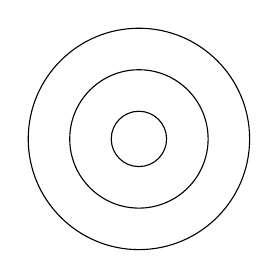
\begin{tikzpicture} 
         \draw (0,0) circle (40pt);
         \draw (0,0) circle (25pt);
         \draw (0,0) circle (10pt);
      \end{tikzpicture}
  \end{center}
    \begin{enumerate}[(a)]    
    \item $\frac{1}{10}$
    \item $\frac{1}{4}$
    \item $\frac{4}{7}$
    \item $\frac{1}{2}$
    \item $\frac{3}{4}$
    \end{enumerate}
      \begin{sol}
        resposta: e \\
        Área pedida: $\pi(8^2-4^2)=48\pi\Longrightarrow p= \frac{48\pi}{64\pi}=\frac{3}{4}$
      \end{sol}
\end{ex}